\documentclass[a4paper,12pt,onecolumn]{article}

\usepackage[english]{babel}
\usepackage{amssymb,amsmath,array,epsfig,a4,subfig}


\newcommand{\errorXx}{\|\Gamma^h - \Gamma\|_{L^\infty}}
\newcommand{\LerrorUu}[1]{\|\vec U - I^h_{#1}\,\vec u\|_{L^2(\Omega_T)}}
\newcommand{\errorUu}[1]{\|\vec U - I^h_{#1}\,\vec u\|_{L^\infty}}
\newcommand{\errorPp}[1]{\|P - I^h_{#1}\,p\|_{L^\infty}}
\newcommand{\LerrorPp}{\|P - p\|_{L^2(\Omega_T)}}

\begin{document}

\captionsetup[subfigure]{labelformat=empty} % remove label subplot
\newcolumntype{H}{>{\setbox0=\hbox\bgroup}c<{\egroup}@{}} % hide table column

\section{Miscellaneous}

Fluid flow problems with a moving interface are encountered in many
applications in physics, engineering and biophysics. Developing robust and
efficient numerical methods for these flows is an important problem and
has attracted tremendous interest over the last decade. Apart from the usual
difficulties arising from the numerical computation of the fluid flow in the
bulk, the accurate approximation of the moving free interface, as well as a
suitable description of the conditions that need to hold on the interface,
pose serious challenges. Of particular importance is the precise inclusion of
surface tension terms, and the correct handling of discontinuity jumps in the
material properties and in the pressure at the interface, in order to suppress
spurious velocities, which are also called parasitic currents.

In this paper we propose a novel finite element approximation for
incompressible two-phase Stokes flow that naturally avoids spurious
velocities. Our scheme is based on the numerical method introduced in
\cite{spurious}, and so uses piecewise linear parametric finite elements to
describe the moving discrete interface. In contrast to \cite{spurious}, where
the interface and the bulk mesh were totally independent, here we pursue the
fitted approach. That means that the interface discretization is always fitted
to the bulk mesh, i.e.\ the discrete interface is made up of edges/faces of
elements belonging to the bulk mesh. An advantage of our method is that the
discontinuity jumps in the material properties and in the pressure are captured
naturally. In particular, we do not need to employ an XFEM-type extension of
standard bulk pressure spaces. Surface tension forces are discretized with the
help of a variational approximation of curvature that was first proposed in
\cite{triplej,gflows3d}. Combining this with an implicit treatment of the
surface tension forces yields an unconditionally stable scheme. Interestingly,
the formulation of curvature from \cite{triplej} leads to a tangential motion
of vertices in practice, which guarantees equidistribution in 2d and good
meshes in 3d. Overall, our proposed method has the following properties.
\begin{itemize}
\item The fully discrete scheme is unconditionally stable in the sense that the
total surface energy is monotonically decreasing independent of the chosen time
step size.
\item In the absence of outer forces, any discrete solution with a stationary
interface must have zero velocity globally, i.e.\ we can prove that there are
no stationary solutions with spurious velocities. Similarly, discrete
stationary solutions for spherical interfaces are attained for our scheme.
\item For the semidiscrete continuous-in-time variant of the fully discrete
scheme the volume
of the two phases is conserved. The fully discrete scheme itself maintains the
enclosed volumes well in practice.
\item Thanks to the fitted nature of the finite element method, the pressure
jumps at the interface are captured accurately for standard pressure finite
element spaces without the need for XFEM extensions.
\item The surface tension effects are included with the help of a variational
treatment of curvature based on the Laplace--Beltrami operator.
\item The surface mesh quality is maintained. In particular, for the
semidiscrete scheme an equidistribution property can be shown in 2d.
\item The fully discrete scheme uses an implicit approximation of curvature
that leads to a coupled linear system of equations to be solved at each time
step.
\end{itemize}

Let us briefly discuss alternative approaches to the numerical approximation of
two-phase flow problems. In this paper we use a direct description of the
interface.  In such direct
approaches, which are often called front-tracking methods, the interface is
either triangulated or presented by a connected set of particles. The discrete
interface is advected with the help of the bulk fluid velocities, and
quantities on the interface need to be suitably coupled to the bulk equations.
In our situation, a finite element parameterization of the unknown interface
is employed.
We refer e.g.\ to
\cite{UnverdiT92,Bansch01,Tryggvason_etal01,GanesanMT07,GanesanT08,spurious}
for further details on front tracking methods,
and to \cite{LevequeL97,Peskin02} for the related immersed
boundary method. Another class of approaches is based on interface capturing
methods using an indicator function to describe the interface. The volume of
fluid (VOF) method and the level set method fall into this category. In the
former, the characteristic function of one of the phases is approximated
numerically, see e.g.\ \cite{HirtN81,RenardyR02,Popinet09}; whereas in the
latter, the interface is given as the level set of a function, which has to be
determined, see e.g.\ \cite{SussmanSO94,Sethian99,OsherF03,GrossR07}.
Finally, in phase
field methods the interface is assumed to have a small, but positive, thickness
and an additional parabolic equation, defined in the whole domain, has to be
solved in these so-called diffuse interface models. We refer to
\cite{HohenbergH77,AndersonMW98,LowengrubT98,Feng06,KaySW08,AbelsGG12,GrunK14}
for details.

\begin{figure}[htbp]
\centering
\includegraphics[width=.45\textwidth]
{figures/2d_stationary_bubble_adaptive_100.ps}
\caption{($\mu=\gamma=1$) Pressure of the 2d stationary bubble at time $t=1$
for the P2--P0 element.}
\end{figure}

\begin{figure}[htbp]
  \centering
  \subfloat[$t=0$]{\includegraphics[width=.45\textwidth]
  {figures/expanding_bubble_uniform_000.ps}}\\
  \subfloat[$t=0.25$]{\includegraphics[width=.45\textwidth]
  {figures/expanding_bubble_uniform_025.ps}}
  \subfloat[$t=0.5$]{\includegraphics[width=.45\textwidth]
  {figures/expanding_bubble_uniform_050.ps}}\\
  \subfloat[$t=0.75$]{\includegraphics[width=.45\textwidth]
  {figures/expanding_bubble_uniform_075.ps}}
  \subfloat[$t=1$]{\includegraphics[width=.45\textwidth]
  {figures/expanding_bubble_uniform_100.ps}}
\caption{($\mu_+ = 10\,\mu_- = \gamma = 1,\alpha = 0.15$) Pressure evolution of
the 2d expanding bubble for the P2--P0 element, $C_r=3$.}
\end{figure}

In order to choose the better remeshing coefficient $C_r$ several experiment
were carried out. Some errors for our approximation are shown in
Table~\ref{tab:expandingbubble2Dp2p0bothdiffcr} with a starting characteristic
length $c_l=0.1$, using P2--P0 polynomials and smoothing coefficient $C_s=1$.
The better result are obtained with $C_r=3$ because it reduces the number of
remeshing compared to $C_r=2$ while keeping the same performance and error
quality. For this reason we are going to use this parameter for the other
simulations.
\begin{table*}
 \center
\begin{tabular}{llHllHll}
\hline
$C_r$ & $\errorXx$ & $\LerrorUu2$ & $\errorUu2$ & $\LerrorPp$ & $\errorPp0$ &
$CPU[s]$ & $K_\Omega^T$\\
\hline
2 & 1.46658e-03 & 1.05801e-04 & 8.73227e-04 & 2.14589e-01 & 3.68834e-02 & 4297
& 452\\
3 & 1.47162e-03 & 1.02085e-04 & 7.19650e-04 & 2.13599e-01 & 3.68834e-02 & 3919
& 468\\
4 & 1.46761e-03 & 1.27330e-04 & 8.55458e-04 & 2.19071e-01 & 3.68834e-02 & 4682
& 504\\
5 & 1.47218e-03 & 1.26419e-04 & 7.20711e-04 & 2.12456e-01 & 3.68834e-02 & 4775&
468\\
\hline
\end{tabular}
\caption{($\mu_+ = 10\,\mu_- = \gamma = 1,\alpha = 0.15$) Expanding bubble
problem on $(-1,1)^2\setminus[-\frac{1}{3},\frac{1}{3}]^2$ over the time
interval $[0,1]$ for the P2--P0 element, $C_s=1$, $c_l=0.1$ and uniform mesh.}
\label{tab:expandingbubble2Dp2p0bothdiffcr}
\end{table*}

In all the previous simulations, the meshes used were uniform therefore the
characteristic length was equal for all the nodes. Moreover they were kept
uniform also after the remeshing. Obviously, with this approach, it is very
expensive to have a large number of interface elements since it leads to a
drastic increase of bulk elements. In the following simulations, instead, we use
adaptive meshes which are fine close to the interface and coarse far from the
interface.

Instead, in Figure~\ref{fig:shear_2d_smooth} the remeshing coefficient is
$C_r=0$ so only the smoothing is used. The bulk inner relative volume evolution
is reported in Figure~\ref{fig:shear_2d_smooth_bulk_inner_volume}.
\begin{figure}[htbp]
  \centering
  \subfloat[$t=0.5$]{\includegraphics[width=.45\textwidth]
  {figures/2d_shear_smooth_050.ps}}\quad
  \subfloat[$t=1$]{\includegraphics[width=.45\textwidth]
  {figures/2d_shear_smooth_100.ps}}\\
  \subfloat[$t=2.5$]{\includegraphics[width=.45\textwidth]
  {figures/2d_shear_smooth_250.ps}}\quad
  \subfloat[$t=5$]{\includegraphics[width=.45\textwidth]
  {figures/2d_shear_smooth_500.ps}}\\
  \caption{($\mu=1,\gamma=3$) Pressure evolution of the 2D shear flow with
$c_l=0.05$, $C_s=1$ and no remeshing for the P2--P0 element, uniform mesh.}
  \label{fig:shear_2d_smooth}
\end{figure}

\begin{figure}[htbp]
  \centering
  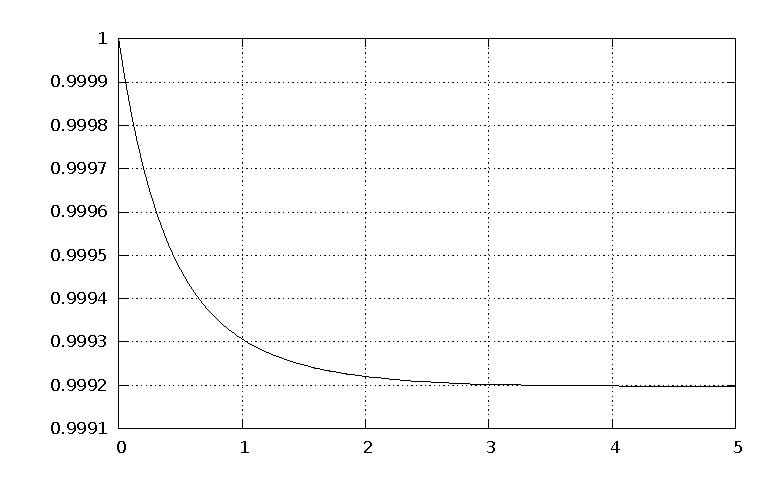
\includegraphics[width=.45\textwidth]
  {figures/2d_shear_smooth_bulk_inner_volume.ps}
  \caption{($\mu=\gamma=1$) Bulk inner relative volume evolution of the 2D
shear flow with $c_l=0.05$, $C_s=1$ and no remeshing for the P2--P0 element,
uniform mesh.}
  \label{fig:shear_2d_smooth_bulk_inner_volume}
\end{figure}

TODO : add comparison reults unfitted scheme scheme stokes paper

The P2--P0 element has the same accuracy of the P2--(P1+P0) element but it is
simpler to implement, always satisfies the LBB condition and the resulting
linear system is smaller therefore it is the best choice.

The adaptive mesh works very well for the stationary bubble problem. Indeed,
with a fraction of bulk elements, it reaches the same accuracy of the uniform
mesh. Unfortunately this is not the case for the expanding bubble problem. For
this problem, the uniform mesh is much faster and requires less bulk elements
compared to the adaptive mesh therefore.\footnote{But they have different
$\tau$!}

In the 2D expanding bubble problem, We can observe that the simulations which
use only the smoothing have bigger errors and take more time therefore it is not
feasible to use only the smoothing process. On the other side both only
remeshing and smoothing/remeshing combined achieve almost the same quality and
performance. It is important to notice that the performance are almost the same
for sequential code (our case) but in parallel computation the remeshing is the
real bottleneck therefore it is way better to use the combined
smoothing/remeshing approach.

Both element capture perfectly the jump in the pressure.

We have presented a novel fitted finite element approximation for two-phase
Stokes flow. The method uses a piecewise linear approximation of the interface
and employs standard velocity and pressure finite element spaces in the bulk.

The scheme is unconditionally stable and can capture simple stationary
solutions exactly, which means that no spurious velocities appear. In addition,
the discontinuous pressure jumps are captured well in general situations, and
no pressure oscillations appear in practice.

Moreover, the numerical solutions exhibit good volume conservation properties
and the quality of the interface mesh does not deteriorate in time.

\end{document}
